% 2007 年四川卷文科第 14 题：题图。
% 来源 PDF：普通高考/2007/2007四川文.pdf，SHA256 1318df44733ec939e8789379d6fa2115a2c6a63e84b73c1f2bf3c080007ce68c
% 原页：第 1 页（A3 三栏）第 3 栏，印刷页 411，图在题干下方。
% 重绘依据：竖放正三棱柱斜二测画法，侧棱与底面边长之比按 √2:1；可见棱实线、不可见棱与 BC1 虚线；与文科原页比对一致。
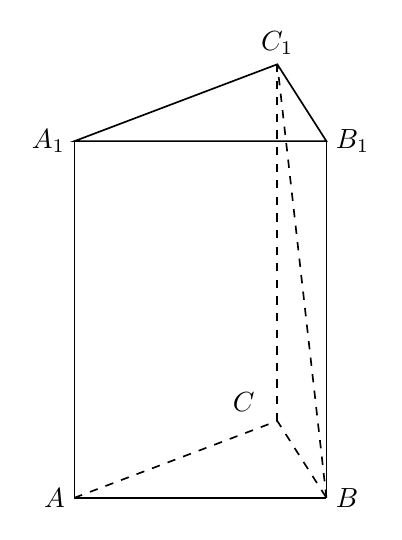
\begin{tikzpicture}[scale=1.6, semithick,
  every node/.style={inner sep=1.5pt}]
  \coordinate (A1) at (0,0);
  \coordinate (B1) at (2,0);
  \coordinate (C1) at (1.61,0.61);
  \coordinate (A)  at (0,-2.83);
  \coordinate (B)  at (2,-2.83);
  \coordinate (C)  at (1.61,-2.22);
  % 不可见的三条棱与辅助线
  \draw[dashed] (A) -- (C) -- (B);
  \draw[dashed] (C) -- (C1);
  \draw[dashed] (B) -- (C1);
  % 可见的侧棱与底边
  \draw (A1) -- (A);
  \draw (B1) -- (B);
  \draw (A) -- (B);
  % 上底
  \draw (A1) -- (B1) -- (C1) -- cycle;
  \node[anchor=east] at ([xshift=-1pt]A1) {$A_1$};
  \node[anchor=west] at ([xshift=1pt]B1) {$B_1$};
  \node[anchor=south] at ([yshift=1pt]C1) {$C_1$};
  \node[anchor=east] at ([xshift=-1pt]A) {$A$};
  \node[anchor=west] at ([xshift=1pt]B) {$B$};
  \node[anchor=south east] at ([xshift=-4pt,yshift=1pt]C) {$C$};
\end{tikzpicture}
